\chapter{ATP: The Energy-Currency Analogy and Its Limits}

\begin{kaichang}
Before turning the page, fetch a sugar cube from the kitchen, or a spoonful of white sugar. Put it on the table, look at it, and answer three questions.

First, how much do you think all the ATP in your body---the ``energy currency'' of biology textbooks---weighs? Second, how much ATP will you use today? Third, how long, on average, does an ATP molecule ``live'' between being made and being used?

Here are the answers: all your ATP totals about 50 grams, not enough to cover a palm, but the total used today approaches your body mass---tens of kilograms. Each molecule lasts only a minute or two between being ``printed'' and ``spent.''

These numbers sound contradictory. Tens of kilograms spent with only 50 grams in hand? Unless each molecule is reused over a thousand times. The sugar on the table is raw material for this frantic machine of printing, spending, and printing again. We will explore how it works, and why the textbook phrase ``breaking a high-energy phosphate bond releases energy'' is fundamentally wrong.
\end{kaichang}

\section{A Puzzle: Sugar Cannot Be Stuffed into Muscle}

Start with visible facts. The sugar, rice, and noodles you eat mostly become glucose (Chapter 46) entering blood. Climbing stairs, blinking, heartbeat, and thought all require energy ultimately traced to food. ``Sugar is fuel'' is correct.

Yet something is puzzling on reflection. Muscle contraction, nerve firing, a firefly's light, and calcium pumping into cellular stores all need energy in apparently different forms, while sugar is just one thing. A sugar molecule cannot climb inside myosin, Chapter 48's protein motor, and burn on the spot, can it?

Consider burning sugar outside the body. Imagine lighting a sugar cube---do not actually try; it is hard to ignite. Glucose reacts with oxygen to give the same products as inside you: carbon dioxide and water. But combustion outside turns energy \textbf{all at once into heat}, gone in a flash. You ``burn'' sugar quite rapidly: an adult releases as much daily energy as a hundred-watt lamp running all day. Yet you neither heat to a hundred degrees nor glow. Where did the energy go?

Cells never release it all at once. They divide glucose's ``large-denomination deposit'' into small change, handing one piece at a time to a particular working molecular machine. That change is ATP.

\section{Zooming In on an ATP Molecule}

ATP stands for adenosine triphosphate. Its name reveals the structure: adenosine trailing three phosphates.

Adenosine itself combines a nitrogen-containing ring structure, adenine (you will meet it again in DNA in a few years as the genetic alphabet's A), with a five-carbon sugar, ribose, whose relatives appeared in Chapter 46. Three phosphate groups trail behind like fruit on a skewer, each with a phosphorus core surrounded by four oxygens.

Here is the crucial detail: at cellular pH, about 7, these three phosphates carry roughly four negative charges in total. Recall Chapter 9's electrostatic rule: like charges repel, more strongly at shorter distances. Four negative charges crowded onto a short tail resemble identical poles of four magnets forced into one railway car, each trying to get farther from the others.

\begin{center}
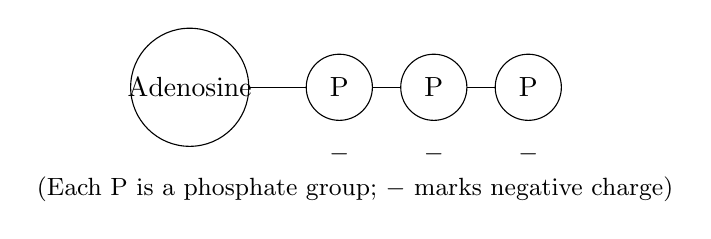
\begin{tikzpicture}
\draw (0,0) circle (0.75) node {Adenosine};
\draw (1.9,0) circle (0.42) node {P};
\draw (3.1,0) circle (0.42) node {P};
\draw (4.3,0) circle (0.42) node {P};
\draw (0.75,0) -- (1.48,0);
\draw (2.32,0) -- (2.68,0);
\draw (3.52,0) -- (3.88,0);
\node at (1.9,-0.85) {\small $-$};
\node at (3.1,-0.85) {\small $-$};
\node at (4.3,-0.85) {\small $-$};
\node at (2.1,-1.3) {\small (Each P is a phosphate group; $-$ marks negative charge)};
\end{tikzpicture}
\end{center}

This is a human-drawn schematic: circle sizes are not to scale, and actual molecular shape requires experimental measurement. But it captures a real feature, the tail's crowded negative charges. Remember this picture; there will be a test.

\section{Energy Is Not Inside Any One Bond}

Now dismantle the most widespread mistaken statement. Popular science books and even some textbooks say, ``ATP has a terminal high-energy phosphate bond that releases energy when broken.'' It sounds reasonable: a bond stores energy like a compressed spring, which springs out when cut to drive life.

Unfortunately, this directly contradicts chemistry's basic accounts. Chapter 27 established that \textbf{breaking any chemical bond absorbs energy; forming bonds releases it}, without exception. If breaking bonds released energy, continuously dismantling molecules would generate energy from nothing, and perpetual-motion machines would already exist. ATP hydrolysis does break bonds, so that step necessarily \textbf{absorbs} energy and cannot be its source.

Where, then, does hydrolysis's genuine energy release come from? Count the whole reaction, not only bond breaking. ATP reacts with water to form ADP, adenosine diphosphate with one fewer phosphate, plus free inorganic phosphate. Two main credits explain the net release.

First, \textbf{products are much more stable than reactants}. The previously crowded negative charges split between two independent molecules---ADP taking a little over two and phosphate two---which can separate freely in water, reducing repulsion. Free phosphate also gives electrons more ways to delocalize (resonance, Chapter 19), while water surrounds the products (solvation, Chapter 25), lowering energy further. Bond formation, dispersal, and water's embrace release more energy together than bond breaking costs.

Second, more subtly, \textbf{cells maintain ATP and ADP concentrations far from equilibrium}. Recall Chapter 31: every reversible reaction has an equilibrium where forward and reverse accounts balance and no energy can be extracted. ATP hydrolysis strongly favors products; ATP dissolved in water and left alone would eventually almost all become ADP and phosphate. Cells constantly oppose this direction, spending energy to remake ATP and keep its concentration far above equilibrium. Like pumps filling an elevated reservoir day and night, they maintain stored energy not in ATP alone but in the \textbf{concentration difference between ATP and ADP}, formally called chemical potential. The water-level difference generates electricity, not water itself.

\begin{qiaoliang}
Estimate the scale. Under standard conditions, ATP hydrolysis releases about \ud{30.5}{kJ} of free energy per mole; cellular high ATP and low ADP increase this to about \ud{50}{kJ/mol}. An adult uses about \ud{8000}{kJ} daily. If it all passed through ATP, this would require $8000 \div 50 = 160$ moles. At ATP's molar mass of about \ud{507}{g/mol}, that is roughly 80 kilograms, the same order as body mass and the origin of the opening estimate. Yet actual ATP totals only about 0.1 mole, or 50 grams. Divide: every molecule cycles over a thousand times daily. ATP is not an energy warehouse, but a very fast conveyor belt.
\end{qiaoliang}

\section{Symbols: How the Currency Is Spent}

We have waited this long for chemical notation because symbols must grow from understanding. Biochemists abbreviate ATP hydrolysis as:

\[\chem{ATP} + \chem{H_2O} \rightarrow \chem{ADP} + \chem{P_i}\]

$\chem{P_i}$ denotes inorganic phosphate. This is shorthand: real dissolved species are charged, with proton changes too. A rigorous version is $\chem{ATP^{4-}} + \chem{H_2O} \rightarrow \chem{ADP^{3-}} + \chem{HPO_4^{2-}} + \chem{H^+}$. Notice that the reaction also releases a little acid, handled by cellular buffers (Chapter 32).

This shorthand contains the secret of currency production and circulation: spend it in one direction, print it in the other. Where does the analogy work? In three particularly vivid ways.

First, \textbf{universality}. Glucose breakdown, fat oxidation, and sunlight in plants supply income, all exchanged first for ATP. Muscle contraction, ion pumping, protein synthesis, and firefly light pay expenses with ATP. Earners and spenders need not know one another, just as your casual employer needs no agreement with the convenience store downstairs. Without this intermediary, every energy-releasing reaction would need separate wiring to every energy-requiring process, impossible to coordinate among tens of thousands of cellular reactions.

Second, \textbf{suitable denominations}. Complete oxidation of one mole of glucose releases about \ud{2800}{kJ}. Releasing it all at once yields a heat wave useless for delicate tasks. ATP-sized portions, about \ud{50}{kJ/mol}, are just enough for a conformational change, pumping an ion, or attaching an amino acid. A large banknote is awkward to change; small coins buy a bus ride.

Third, most elegantly, \textbf{phosphate can be transferred directly}. Often ATP does not hydrolyze and scatter energy; it transfers its entire terminal phosphate to another molecule, phosphorylation. Glucose receives one immediately after entering a cell (Chapter 52's first step). Its reactivity changes completely: it becomes more reactive and easier for the next enzyme to process. The added negative charge also prevents escape through the membrane (Chapter 51), effectively registering and detaining it inside. No mysterious energy flows into glucose; a concrete group transfer rewrites the overall account into a favorable direction.

\section{How Scientists Know: Muscle Contraction in a Test Tube}

\begin{zhengju}
Early twentieth-century researchers knew vigorous muscle activity produced lactic acid (Chapter 52), suggesting that a glycolytic product directly powered contraction. In the late 1920s, Danish physiologist Lundsgaard conducted an elegant elimination experiment: iodoacetic acid completely blocked glycolysis in muscle, yet it still contracted several times. Glycolysis itself was not the immediate fuel; another ready reserve existed. Phosphocreatine was soon discovered, and in 1929 Lohmann isolated a substance containing adenine and three phosphates---ATP.

What did ATP do? In 1939, Engelhardt and Lyubimova found that the motor protein myosin was itself an ATP-hydrolyzing enzyme (Chapter 49): fuel and engine met in one machine. The decisive result came from Szent-Györgyi's laboratory. Extracted actin and myosin were mixed in a test tube and drawn into threads to form artificial muscle. The threads lay still without reactants; add ATP, and they contracted. For the first time, a lifeless test tube containing two purified proteins and a small molecule reproduced movement, that most lifelike activity.

Skeptics asked whether ATP was merely a structural component or impurities were responsible. Later experiments showed strict correspondence between contraction and ATP-hydrolysis rates; replacing ATP with a similar but nonhydrolyzable molecule left the threads motionless. In 1941, Lipmann assembled the scattered facts into the general picture of ATP as every cell's common energy intermediary. For convenient notation, he introduced ``$\sim$P'' for a high-energy phosphate bond. The notation remains in textbooks, though Lipmann understood that energy was not inside the bond. Later physical chemists repeatedly clarified the net release from more stable products and concentrations far from equilibrium, but the correction never traveled as far as the wavy line. Remember this: an analogy can be useful and misleading simultaneously. Science corrects it by defining its scope, not necessarily discarding it.
\end{zhengju}
\section{Joining Energy Release to Energy Demand}

One connection needs full explanation: how are ATP hydrolysis's release and muscle contraction's demand joined? Not by hydrolyzing ATP first, releasing energy into the cell, and letting another machine collect it. Once dispersed as heat, energy cannot be retrieved that way. Hot water can do work because of its temperature difference from the surroundings, not heat alone. At uniform cellular temperature, heat is unusable money.

The real connection is \textbf{reaction coupling}: an enzyme binds favorable and unfavorable half-reactions into one event. In myosin, Chapter 48's protein motor, ATP first binds the active site. Hydrolysis's free energy does not scatter but directly changes the protein's shape, like cocking a mousetrap. Myosin then transmits that shape change to actin, producing a sliding step. Release and work occur in the same molecular action, with energy never leaving the account as heat.

Car engines offer a contrast: efficiency is only twenty or thirty percent because chemical energy first becomes heat, then motion, paying a heavy thermodynamic tax (Chapter 28). Cells bypass heat, converting chemical energy directly into chemical energy or mechanical deformation, so muscle efficiency can be much higher. Much food energy ultimately becomes body heat, but that is unspendable change, not the payment mechanism itself.

\textbf{Translator safety note:} Use a low-power visible blue-light torch for this activity, not an unknown UV source or a germicidal UVC lamp. An arm's-length distance alone does not establish UV safety; avoid exposure of eyes and skin. See \href{https://www.fda.gov/radiation-emitting-products/tanning/ultraviolet-uv-radiation}{FDA UV guidance}.

\begin{shiyan}
\textbf{Watch an Electron Currency's Raw Material Glow.} Later we will meet cellular armored cars carrying electrons alongside ATP. One, FAD, has a core derived from vitamin B2, riboflavin, the inexpensive little yellow pharmacy tablets. You can see an energy trick of this molecule.

Materials: a vitamin B2 tablet, warm water, a clear glass, a small UV banknote-checking torch (or blue-light torch), and a room that can be darkened.

Steps: crush the tablet into warm water and stir until the water is pale yellow. Darken the room and illuminate the glass from the side, keeping your eyes an arm's length from the lamp.

What to observe: illuminated water gives bright yellow-green fluorescence. Molecules absorb higher-energy ultraviolet and emit lower-energy yellow-green light, making change by wavelength rather than losing energy. Turn off the lamp and fluorescence stops immediately: molecules transfer light, not store it. Inside cells, FAD does not shine yellow; it uses its energy-accepting ability to catch electrons, the real transport business.

Safety note: never aim UV at eyes or expose skin for long. Do not drink this water; wash hands and put tablets away afterward.
\end{shiyan}

\section{Where the Currency Analogy Breaks Down}

Now fulfill the title's other promise: where the analogy \textbf{fails}. A misused analogy can be worse than none, so remember four limits.

First, \textbf{money can be saved; ATP cannot}. Coins sit in a piggy bank for ten years; cellular ATP is spent within a minute or two. Real savings are glycogen and fat (Chapters 46 and 47), while ATP is cash flow. Muscle does have a little change jar, phosphocreatine, rapidly recharging ADP in the first seconds of intense exercise---the principle behind athletes' creatine supplementation. But its supply lasts only tens of seconds, not a treasury.

Second, \textbf{money's buying power seems fixed; ATP's fluctuates}. A ten-unit banknote is ten units today and tomorrow, while ATP hydrolysis's free-energy yield depends on ATP, ADP, and phosphate concentrations. When cellular energy is tight and ADP accumulates, the same ATP becomes more valuable, as if banknote denominations varied with bank reserves. The challenge supplies calculations.

Third, \textbf{money spent is gone; ATP cycles}. This is the biggest difference. After hydrolysis to ADP and phosphate, fresh fuel energy promptly rebuilds ATP. What is truly spent is glucose's chemical potential; ATP circles through charging and discharging. Strictly, it is more a rechargeable power bank than a coin: your daily tens of kilograms spent are a 50-gram power bank cycling over a thousand times.

Fourth, \textbf{ATP is not the only currency, and some energy bypasses it}. At least two parallel payment systems exist. One uses \textbf{electron carriers}, NADH and FADH$_2$ (written $\chem{NADH}$ and $\chem{FADH_2}$), carrying high-energy electrons rather than phosphate. As Chapter 33 explained, gaining electrons is reduction: $\chem{NAD^+}$ accepts two electrons and a proton from glucose fragments to become $\chem{NADH}$, like an armored car taking cash to the mitochondrial vault, opened in Chapter 53. The experiment's fluorescent riboflavin is $\chem{FAD}$'s core. The other system is stranger: \textbf{a concentration gradient itself is energy}. Cells pump protons to one membrane side, establishing concentration and electrical-potential differences, together the proton-motive force. Like reservoir filling or battery charging (Chapter 34), maintaining imbalance stores energy without a special molecule. Chapter 53 will show that most cellular ATP is printed by proton flow through a membrane motor.

The real picture is richer than currency alone: change (ATP), armored cars (NADH and FADH$_2$), reservoirs (proton gradients), and deposits (glycogen and fat). The analogy is a map, not the territory.

\begin{wuqu}
``Exercise uses energy by continually breaking ATP's high-energy phosphate bonds.'' Wrong on every level. First, breaking bonds always absorbs energy. Net hydrolysis release comes from ADP and phosphate's greater stability, charge dispersal, resonance, solvation, and ATP concentration maintained far above equilibrium. Second, even favorable hydrolysis alone drives no activity: pour ATP into water, and you obtain only slightly warmer water. Using the energy requires enzyme coupling of hydrolysis and work within the same molecular action. Third, ``high-energy bond'' is a notation inherited from 1941, the wavy $\sim$P, indicating what phosphate transfer can drive, not an energy-filled spring. A counterexample is readily available: ATP's phosphorus--oxygen bonds are not unusual compared with ordinary phosphate-ester bonds in the energy required to break them. Laboratory bond-breaking measurements show nothing anomalous. What is unusual is not the bond but the entire system's concentration pattern.
\end{wuqu}

\section{Back to the Sugar on the Table}

Look again: the sugar cube should now appear different.

It is not stuffed into muscle and burned on the spot. Cells import and dismantle it along Chapter 52's production line, using some chemical potential to print a little ATP directly and packing more into NADH for mitochondrial delivery. There, in Chapter 53, electrons descend a chain, powering proton pumps to build a transmembrane reservoir. Returning protons rotate ATP synthase for bulk printing. Within minutes, ATP circulates to change myosin's shape and lift your hand, power ion pumps for nerve firing, drive ribosomes to join amino acids, or occasionally light a firefly. ADP and phosphate return to the printing works for another charge.

The opening numbers now fit: a fast currency flow means small stock (50 grams), large throughput (tens of kilograms daily), and short molecular lifetime (a minute or two). Three contradictions are three faces of one coin. The high-energy-bond story fails by focusing on one design stamped on the coin while missing the reservoir generating power: concentration imbalance is the reservoir of all cellular energy.

\section{Where Are the Printing Works?}

We have examined the spending end and clarified what ATP is and is not, but the printing works remain unexplored. Where in glucose breakdown does the first ATP appear? How do NADH electrons raise the proton reservoir? What does a proton-driven motor turning hundreds of times per second look like? The next three chapters tour the factories: Chapter 52's ancient small-scale glycolytic printer, Chapter 53's high-power mitochondrial machinery, and Chapter 54's solar-powered plant branch. Afterward, this sugar will look like an entire energy industry.

\begin{tiaozhan}
ATP's fluctuating buying power can be calculated. Actual reaction free energy is $\Delta G = \Delta G^{\circ\prime} + RT\ln Q$, where $Q$ is the quotient of product and reactant concentrations. Under standard conditions, each concentration \ud{1}{mol/L}, ATP hydrolysis has $\Delta G^{\circ\prime} \approx \ud{-30.5}{kJ/mol}$. Actual cellular concentrations are about \ud{8}{mmol/L} ATP, \ud{1}{mmol/L} ADP, and \ud{8}{mmol/L} phosphate. Substitute $Q = \dfrac{[\chem{ADP}][\chem{P_i}]}{[\chem{ATP}]} = \dfrac{0.001 \times 0.008}{0.008} = 0.001$. Near body temperature, $RT\ln Q \approx 2.48 \times \ln(0.001) \approx \ud{-17}{kJ/mol}$, giving $\Delta G \approx -30.5 - 17 \approx \ud{-48}{kJ/mol}$. More negative than standard, so cellular ATP buys more than standard ATP. Conversely, fatigue dropping ATP to \ud{4}{mmol/L} and raising ADP to \ud{2}{mmol/L} markedly reduces each ATP's buying power. Life's energy economy has no fixed exchange rate. Skip this without losing the main thread, but following the calculation puts your hand on physical chemistry's door handle.
\end{tiaozhan}

\section*{Exercises}

\begin{sikaoti}
\item Draw ATP--ADP cycling as a material-flow diagram: boxes for ATP and ADP plus phosphate, connected by a loop. Label each arrow with who supplies energy and which molecule or gradient supplies it.
\item Using bond-breaking absorption and bond-formation release, analyze ATP hydrolysis entry by entry: what breaks, what forms, and where should net release be explained? Do not use the phrase ``high-energy bond'' anywhere in your answer.
\item ATP dissolved in water hydrolyzes and releases heat, yet the water performs no work. Explain the missing step compared with cells using reaction coupling, and sketch an enzyme joining favorable and unfavorable half-reactions.
\item Someone needs \ud{8000}{kJ} daily, assumed all passing through ATP at \ud{50}{kJ} per mole and molar mass about \ud{500}{g/mol}. Estimate total daily ATP turnover mass, then compare it with a \ud{50}{g} body stock to estimate cycles per molecule per day.
\item What does $\chem{NAD^+}$ gain on becoming $\chem{NADH}$? Use Chapter 33's redox definition to explain why an electron armored car is more accurate than an energy packet. Where are the electrons ultimately delivered, and what are they exchanged for? The next two chapters reveal this; first write your guess.
\item Ground firefly light organs mixed with water quickly stop glowing. ATP solution restores light; glucose solution does not. Predict and explain all three observations, especially why glucose, the more energetic fuel, fails to light it.

\textbf{Translator safety note:} Treat this as a thought exercise; do not collect or harm fireflies. Use published results or a teacher-selected non-animal demonstration. Collection pressure is among the threats identified in \href{https://xerces.org/endangered-species-conservation/firefly-conservation}{Xerces Society's firefly conservation guidance}.
\end{sikaoti}
